\documentclass[]{article}

% Imports the catppuccin theme, using the mocha flavor,
% from the directory above. Actual implementation
% wouldn't need the import package unless the theme
% and the document are in different directories.
\usepackage{import}
\usepackage{xcolor}
% \usepackage{fancyhdr}
\usepackage{cancel}
\usepackage{mathtools}

% For permutations and combinations
\newcommand\Myperm[2][^n]{\prescript{#1\mkern-2.5mu}{}P_{#2}}
\newcommand\Mycomb[2]{\prescript{#1\mkern-0.5mu}{}C_{#2}}

% Colors
\definecolor{yorhabg}{HTML}{FFFFFF}
\definecolor{yorhafg}{HTML}{000000}
\definecolor{yorhagrid}{HTML}{B5AF9C}
\definecolor{mred}{HTML}{D67069}
\definecolor{mblue}{HTML}{6887A1}

\pagecolor{yorhabg}
\color{yorhafg}

\usepackage{preamble}

% Removes padding above title
\usepackage{titling}
\setlength{\droptitle}{-10em}

% Font package
\usepackage[T1]{fontenc}

\usepackage{fouriernc}

\usepackage{sectsty}
\usepackage{graphicx}
\usepackage{amsmath}
\usepackage{amsfonts}
\usepackage{amssymb}
\usepackage[skins, most]{tcolorbox}
\usepackage{enumitem}

\DeclareMathOperator{\sgn}{sgn}

\usepackage{tikz}
\usepackage{eso-pic}
\usetikzlibrary{calc,shadows.blur}
\usetikzlibrary{angles, quotes}
\usetikzlibrary{3d}

% Margins
\topmargin=0in
\evensidemargin=0in
\oddsidemargin=0in
\textwidth=6.5in
\textheight=9.0in
\headsep=0.25in

\AtBeginEnvironment{tcolorbox}{\small}

\newtcolorbox{imp}{enhanced,arc=0mm,colback=yorhabg,colframe=mred,leftrule=10mm,coltext=yorhafg,%
overlay={\node[anchor=west,outer sep=2pt] at (frame.west) {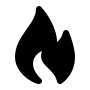
\includegraphics[width=6mm]{images/imageb.png}}; }}

\newtcolorbox{shortcut}{enhanced,arc=0mm,colback=yorhabg,colframe=mred,leftrule=10mm,coltext=yorhafg, coltitle=yorhabg, title=\texttt{Shortcut.}, 
overlay={\node[anchor=west,outer sep=2pt] at (frame.west) {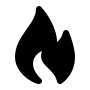
\includegraphics[width=6mm]{images/imageb.png}}; }}

\newtcolorbox{question}[1]{
    enhanced, 
    colback=yorhabg,
    colframe=mblue,
    coltext=yorhafg,
    coltitle=yorhabg,
    attach boxed title to top left={yshift*=-\tcboxedtitleheight}, 
    title=\texttt{#1},
    boxed title size=title,
    boxed title style={%
        rounded corners=northeast, 
        rounded corners=northwest, 
        colback=tcbcolframe, 
        boxrule=0pt,
    },
    underlay boxed title={%
        \path[fill=tcbcolframe] (title.south west)--(title.south east) 
            to[out=0, in=180] ([xshift=5mm]title.east)--
            (title.center-|frame.east)
            [rounded corners=5pt] |- 
            (frame.north) -| cycle; 
    },
}

\newcommand\bb[1]{\textcolor{yorhafg}{\textbf{#1}}}

\title{\textbf{CSCA67 - Exercises \#7}}
\author{Satyajit Datta \ 1012033336}
\date{\today}

\begin{document}

\maketitle
\begin{question}{2.1}
    Prove that $\sqrt{2}$ is irrational.
\end{question}
\begin{flalign*}
    &\text{Suppose } \sqrt{2} \text{ is rational} && (1)\ \text{for contradiction} \\
    &\quad\exists a\exists b, (\sqrt{2} = \frac{a}{b}) \land (a, b \text{ have no common factors} \ne 1.) && (2)\ \text{(1, Definition of $\mathbb{Q}$)}\\
    &\quad(\sqrt{2} = \frac{x}{y}) \land (x, y \text{ have no common factors} \ne 1.) && (3)\ \text{(2, E.I)}\\
    &\quad x^2 =  2y^2 && (4)\ \text{(3, simp. algebra)} \\
    &\quad y^2 \text{ is an integer} && (5)\\
    &\quad \exists k, x^2 = 2k && (6)\ \text{(4, 5, E.G)} \\
    &\quad x^2 \text{ is even} && (7)\ \text{(6, Definition of even)} \\ 
    &\quad x \text{ is even} && (8)\ \text{(7, def., U.M.P)} \\ 
    &\quad x = 2i && (9)\ \text{(8, def. E.I)} \\
    &\quad y^2 = \frac{x^2}{2} = \frac{(2i)^2}{2} = 2i^2 && (10)\ \text{(4, 9)}\\
    &\quad y^2 \text{ is even} && (11)\ \text{(10, def.)} \\
    &\quad y  \text{ is even} && (12)\ \text{(11, def., U.M.P)} \\
    &\quad y = 2j && (13)\ \text{12, def. E.I} \\
    &\quad 2 \text{ is a common factor of} x, y && (14)\ \text{(9, 13)} \\
    &\quad (a, b \text{ have no common factors } \ne 1) && (15)\ \text{(3, simp.)} \\
    &\quad \text{a contradiction}&& (16)\ \text{(14, 15)} \\
    &\sqrt{2} \text{ is irrational.}&& (17)\ \text{(1, 16, contradiction.)}
\end{flalign*}
\begin{center}
    As required to prove. $\blacksquare$
\end{center}

\begin{question}{2.2}
    Prove that the sum of a rational number and an irrational number is irrational.
\end{question}
\[
    WTS: \forall x \forall y, (x \in \mathbb{Q} \land y \notin \mathbb{Q}) \rightarrow ((x+y) \notin \mathbb{Q})
\]

\begin{flalign*}
    &\text{Let a be arbitrary} && (1) \\
    &\text{Let b be arbitrary} && (2) \\
    &\quad\text{Assume $a \in \mathbb{Q}$} && (3) \\
    &\quad\text{Assume $b \notin \mathbb{Q}$} && (4) \\
\end{flalign*}
\begin{center}
    As required to prove. $\blacksquare$
\end{center}
\end{document}